
\documentclass{beamer}
\usepackage[utf8]{inputenc}
\usetheme{Madrid}
\usecolortheme{default}
\usepackage{amsmath,amssymb,amsfonts,amsthm}
\usepackage{txfonts}
\usepackage{tkz-euclide}
\usepackage{listings}
\usepackage{adjustbox}
\usepackage{array}
\usepackage{tabularx}
\usepackage{gvv}
\usepackage{lmodern}
\usepackage{circuitikz}
\usepackage{tikz}
\usepackage{graphicx}
\setbeamertemplate{page number in head/foot}[totalframenumber]
\definecolor{bg}{gray}{0.95}
\lstset{
    language=C,
    basicstyle=\ttfamily\small,
    keywordstyle=\color{blue},
    stringstyle=\color{orange},
    commentstyle=\color{green!60!black},
    numbers=left,
    numberstyle=\tiny\color{gray},
    breaklines=true,
    showstringspaces=false,
}
\title{4.10.3}
\author{Aditya Mishra- EE25BTECH}
\date{September 30, 2025}

\begin{document}

\begin{frame}
\titlepage
\end{frame}

\begin{frame}{Question}
Find the vector equation of the plane passing through the intersection of the planes
\[
\vec{r} \cdot (\hat{i} + \hat{j} + \hat{k}) = 6 \quad \text{and} \quad \vec{r} \cdot (2\hat{i} + 3\hat{j} + 4\hat{k}) = -5,
\]
and the point $(1, 1, 1)$.
\end{frame}

\begin{frame}{Solution}
Given planes:
\[
\vec{n_1}^\top \vec{x} = c_1, \quad \vec{n_2}^\top \vec{x} = c_2,
\]
with point 
\[
\vec{P} = \myvec{p_1 \\ p_2 \\ p_3}.
\]

General form:
\[
\vec{n_1}^\top \vec{x} - c_1 + \lambda(\vec{n_2}^\top \vec{x} - c_2) = 0,
\quad
\lambda = \frac{c_1 - \vec{n_1}^\top \vec{P}}{\vec{n_2}^\top \vec{P} - c_2}.
\]
\end{frame}

\begin{frame}{Solution}

Given:
\[
\vec{n_1} = \myvec{1 \\ 1 \\ 1},\quad c_1 = 6, \quad
\vec{n_2} = \myvec{2 \\ 3 \\ 4},\quad c_2 = -5,
\]
\[
\vec{P} = \myvec{1 \\ 1 \\ 1}.
\]

Evaluate:
\[
\vec{n_1}^\top \vec{P} = 3, \quad \vec{n_2}^\top \vec{P} = 9, \quad \lambda = \frac{3}{14}.
\]
\end{frame}

\begin{frame}{Solution}

Plane equation:
\[
\vec{n_1}^\top \vec{x} - 6 + \frac{3}{14} \left(\vec{n_2}^\top \vec{x} + 5 \right) = 0.
\]
Or
\[
\myvec{\frac{20}{14} \\ \frac{23}{14} \\ \frac{26}{14}}^\top \vec{x} = \frac{69}{14},
\]
which gives integer form
\[
\boxed{
(20 \quad 23 \quad 26) \vec{x} = 69
}.
\]
\end{frame}
\begin{frame}{Plot}
\begin{figure}
    \centering
    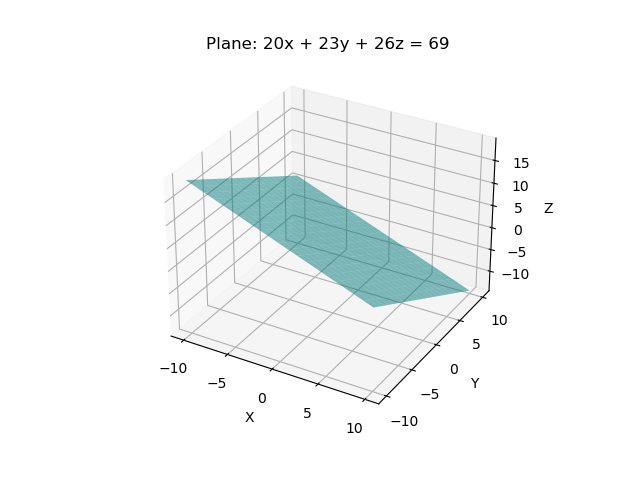
\includegraphics[width=0.8\columnwidth]{Figs/Figure.png}
\end{figure}
\end{frame}

\begin{frame}{Codes}
\centering
For Codes, refer to the URL below:  
\url{https://github.com/Aditya-Mishra11005/ee1030-2025/tree/temp/ee25btech11005/matgeo/4.10.3/Codes}
\end{frame}
\end{document}

